% Architecture figure of M1 (MoE run): quanvolution encoder qconv4x3 + 3 level32 trees + quantum router + per-tree linear heads.
% 2 pages: (1) data flow with parameter counts; (2) quantum router circuit.
% Compile: pdflatex hinh_kien_truc_M1.tex (Overleaf: pdfLaTeX). Labels in English (paper-ready).
% Encoder and tree internals: pages 2-3 of full_quantum_16x16_level32_qconv/hinh_kien_truc_qconv4x3.tex.
% Numbers from models/moe_model.py, models/router.py, test_model.py (Total=17149, quantum 33.75%).
\documentclass[tikz,border=10pt]{standalone}
\usepackage{amsmath,amssymb}
\usetikzlibrary{positioning,arrows.meta,calc,fit,backgrounds,decorations.pathreplacing}

\tikzset{
  >={Stealth[length=2.2mm]},
  qbox/.style={draw=blue!60!black, fill=blue!9, rounded corners=2pt, align=center, font=\small, inner sep=4pt},
  cbox/.style={draw=orange!75!black, fill=orange!13, rounded corners=2pt, align=center, font=\small, inner sep=4pt},
  dbox/.style={draw=black!55, fill=black!4, rounded corners=2pt, align=center, font=\small, inner sep=4pt},
  note/.style={align=left, font=\footnotesize, text=black!75},
  flow/.style={->, thick, black!70},
  gate/.style={draw=blue!60!black, fill=blue!12, minimum width=9mm, minimum height=5mm, inner sep=1pt, font=\scriptsize, align=center},
  meas/.style={draw=blue!60!black, fill=white, minimum width=9mm, minimum height=5mm, inner sep=1pt, font=\scriptsize},
}

\begin{document}

% =====================================================================================================
% PAGE 1: DATA FLOW
% =====================================================================================================
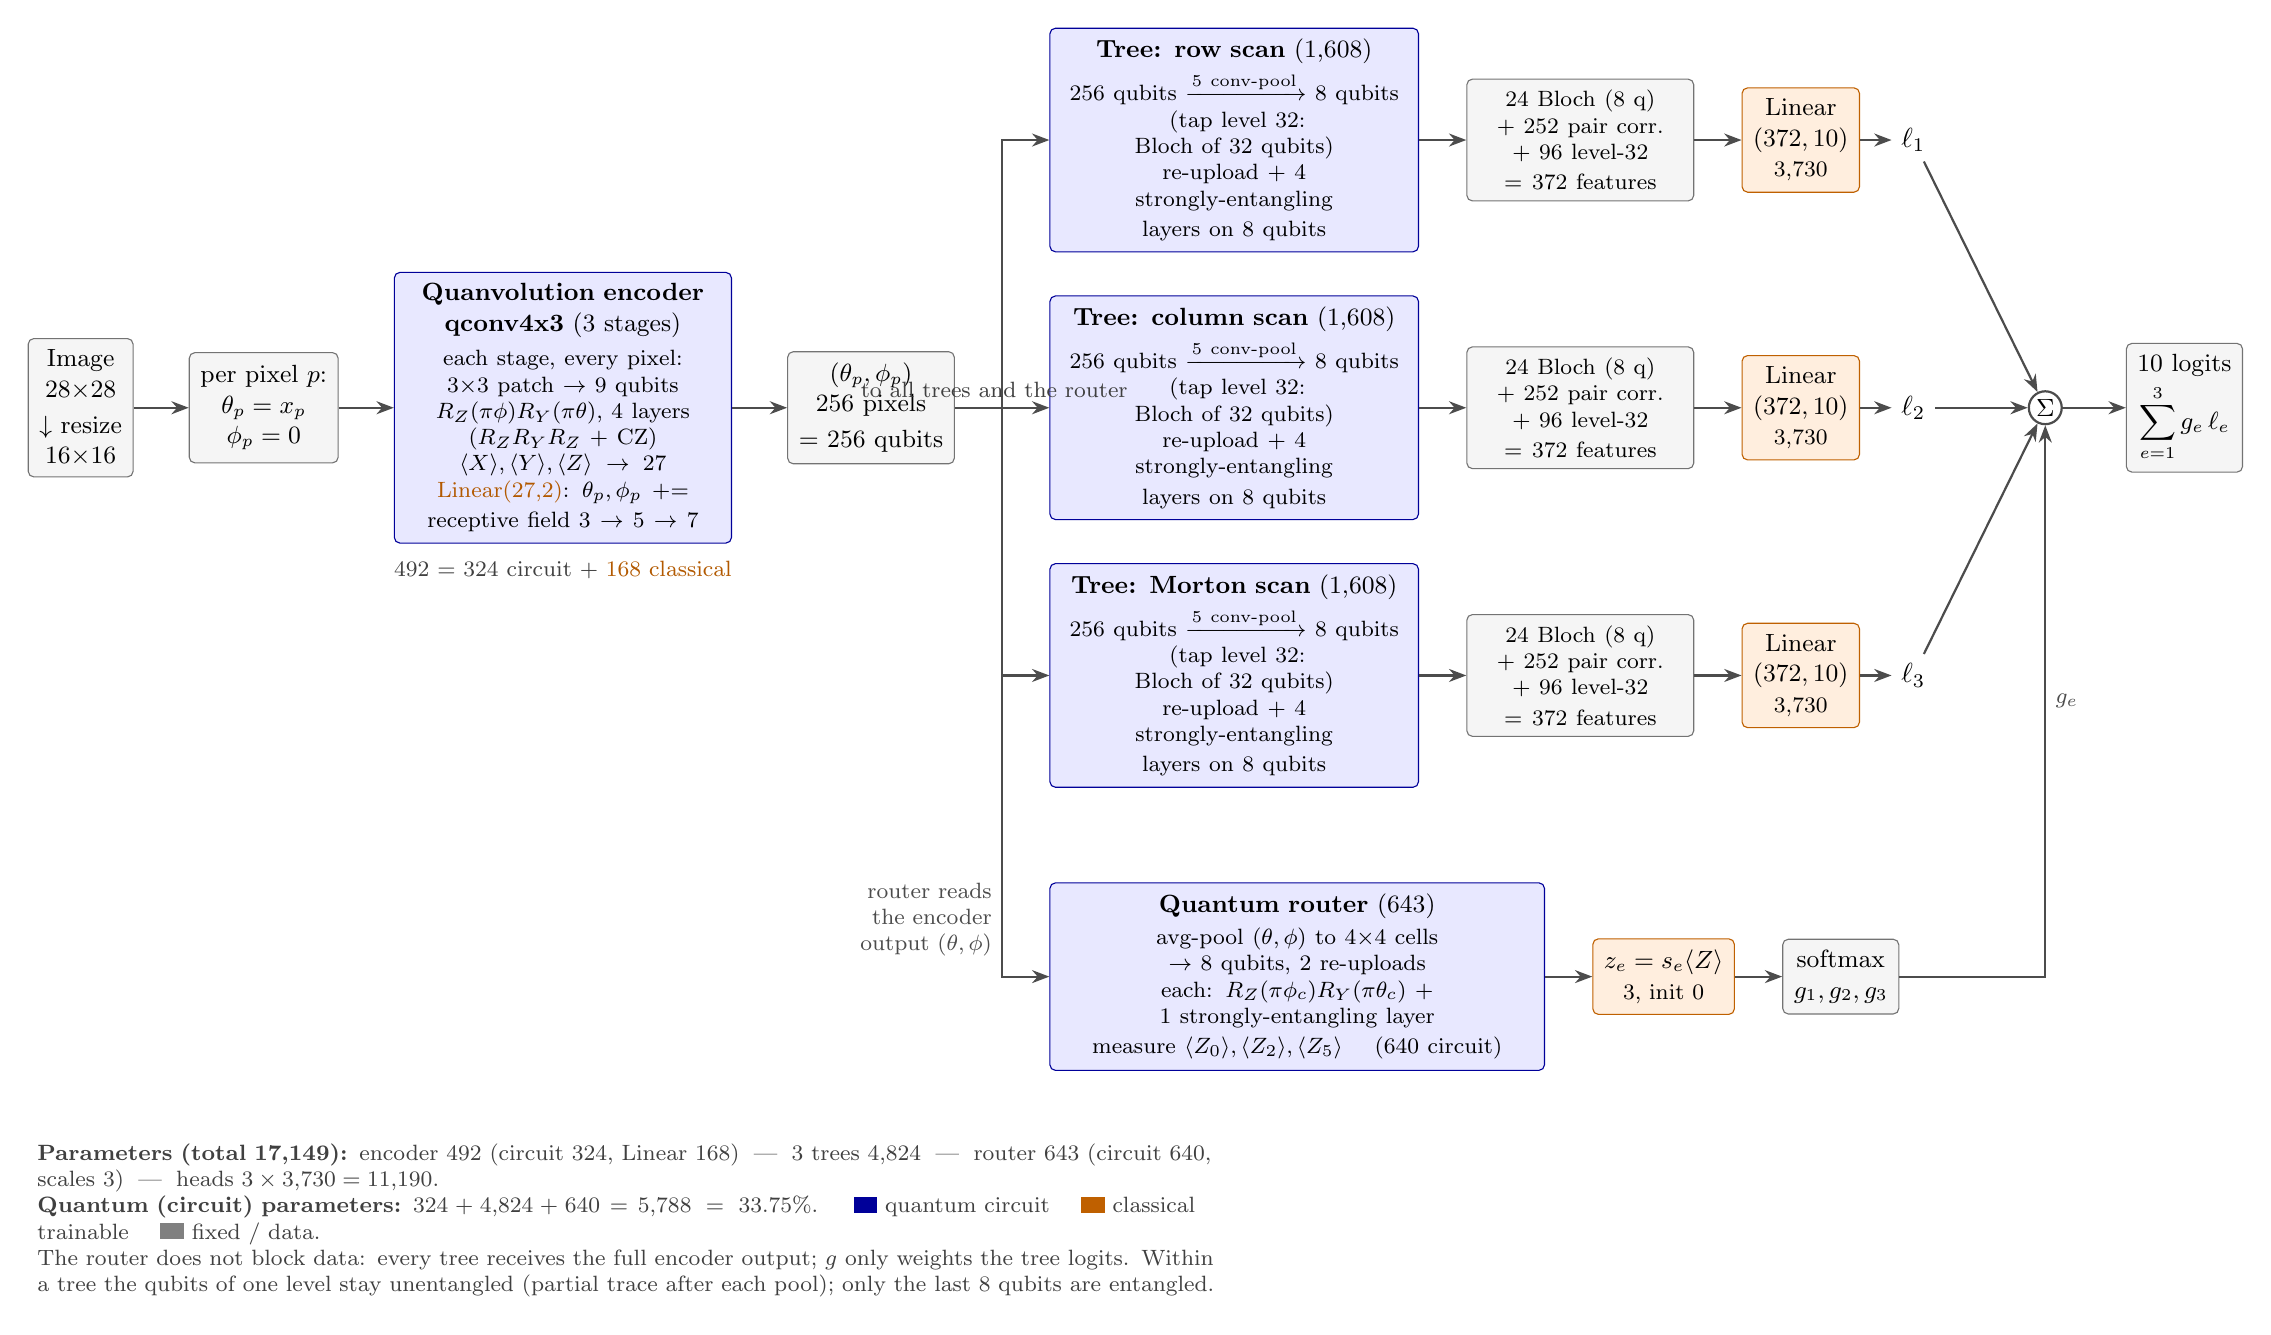
\begin{tikzpicture}[node distance=6mm]

  % ---- input and encoder ----
  \node[dbox, minimum height=14mm] (in) at (0,0) {Image\\$28{\times}28$\\[2pt]$\downarrow$ resize\\$16{\times}16$};
  \node[dbox, right=7mm of in, minimum height=14mm] (init) {per pixel $p$:\\$\theta_p = x_p$\\$\phi_p = 0$};
  \node[qbox, right=7mm of init, text width=40mm, minimum height=30mm] (enc) {%
    \textbf{Quanvolution encoder}\\ \textbf{qconv4x3} (3 stages)\\[3pt]
    \footnotesize each stage, every pixel:\\
    \footnotesize $3{\times}3$ patch $\to$ 9 qubits\\
    \footnotesize $R_Z(\pi\phi)R_Y(\pi\theta)$, 4 layers\\
    \footnotesize ($R_ZR_YR_Z$ + CZ)\\
    \footnotesize $\langle X\rangle,\langle Y\rangle,\langle Z\rangle \to 27$\\
    \footnotesize \textcolor{orange!70!black}{Linear(27,2)}: $\theta_p, \phi_p \mathrel{+}=$\\
    \footnotesize receptive field $3\to5\to7$};
  \node[note, below=1mm of enc] {492 = 324 circuit + \textcolor{orange!70!black}{168 classical}};
  \node[dbox, right=7mm of enc, minimum height=14mm] (tp) {$(\theta_p,\phi_p)$\\$256$ pixels\\[2pt]= 256 qubits};

  % ---- three trees ----
  \foreach \name/\lab/\y in {t0/row/3.4, t1/column/0, t2/Morton/-3.4} {
    \node[qbox, text width=44mm, minimum height=22mm, anchor=west] (\name) at ($(tp.east)+(12mm,\y)$) {%
      \textbf{Tree: \lab\ scan} (1{,}608)\\[2pt]
      \footnotesize 256 qubits $\xrightarrow{\text{5 conv-pool}}$ 8 qubits\\
      \footnotesize \;(tap level 32: Bloch of 32 qubits)\\
      \footnotesize re-upload + 4 strongly-entangling\\
      \footnotesize layers on 8 qubits};
  }
  \foreach \name/\i in {t0/1, t1/2, t2/3} {
    \node[dbox, right=6mm of \name, text width=26mm] (f\i) {\footnotesize 24 Bloch (8 q)\\ \footnotesize + 252 pair corr.\\ \footnotesize + 96 level-32\\ \footnotesize $= 372$ features};
    \node[cbox, right=6mm of f\i] (h\i) {Linear\\$(372,10)$\\\footnotesize 3{,}730};
    \node[right=4mm of h\i] (l\i) {$\ell_{\i}$};
    \draw[flow] (\name) -- (f\i);
    \draw[flow] (f\i) -- (h\i);
    \draw[flow] (h\i) -- (l\i);
  }

  % ---- router ----
  \node[qbox, text width=60mm, minimum height=18mm, anchor=north west] (rt) at ($(t2.south west)+(0,-12mm)$) {%
    \textbf{Quantum router} (643)\\[2pt]
    \footnotesize avg-pool $(\theta,\phi)$ to $4{\times}4$ cells $\to$ 8 qubits, 2 re-uploads\\
    \footnotesize each: $R_Z(\pi\phi_c)R_Y(\pi\theta_c)$ + 1 strongly-entangling layer\\
    \footnotesize measure $\langle Z_0\rangle,\langle Z_2\rangle,\langle Z_5\rangle$ \quad (640 circuit)};
  \node[cbox, right=6mm of rt] (sc) {$z_e = s_e\langle Z\rangle$\\\footnotesize 3, init 0};
  \node[dbox, right=6mm of sc] (sm) {softmax\\$g_1,g_2,g_3$};
  \draw[flow] (rt) -- (sc);
  \draw[flow] (sc) -- (sm);

  % ---- mixture ----
  \node[draw=black!70, circle, thick, inner sep=1pt, font=\small] (mix) at ($(l2.east)+(14mm,0)$) {$\Sigma$};
  \foreach \i in {1,2,3} { \draw[flow] (l\i) -- (mix); }
  \draw[flow] (sm.east) -| node[pos=0.75, right, font=\footnotesize] {$g_e$} (mix.south);
  \node[dbox, right=8mm of mix] (out) {10 logits\\[2pt]$\displaystyle\sum_{e=1}^{3} g_e\,\ell_e$};
  \draw[flow] (mix) -- (out);

  % ---- main arrows ----
  \draw[flow] (in) -- (init);
  \draw[flow] (init) -- (enc);
  \draw[flow] (enc) -- (tp);
  \coordinate (sp) at ($(tp.east)+(6mm,0)$);
  \draw[thick, black!70] (tp.east) -- (sp);
  \foreach \name in {t0,t1,t2} { \draw[flow] (sp) |- (\name.west); }
  \draw[flow] (sp) |- node[pos=0.45, left, font=\footnotesize, align=right] {router reads\\the encoder\\output $(\theta,\phi)$} (rt.west);
  \node[note, above=0mm of sp, xshift=-1mm] {to all trees and the router};

  % ---- legend and counts ----
  \node[note, anchor=north west, text width=150mm] at ($(in.west |- rt.south)+(0,-8mm)$) {%
    \textbf{Parameters (total 17{,}149):}
    encoder 492 (circuit 324, Linear 168) \;|\; 3 trees 4{,}824 \;|\; router 643 (circuit 640, scales 3) \;|\; heads $3\times3{,}730 = 11{,}190$.\\
    \textbf{Quantum (circuit) parameters:} $324 + 4{,}824 + 640 = 5{,}788$ \;=\; 33.75\%. \quad
    \textcolor{blue!60!black}{\rule{3mm}{2mm}} quantum circuit \quad
    \textcolor{orange!75!black}{\rule{3mm}{2mm}} classical trainable \quad
    \textcolor{black!50}{\rule{3mm}{2mm}} fixed / data.\\
    The router does not block data: every tree receives the full encoder output; $g$ only weights the tree logits.
    Within a tree the qubits of one level stay unentangled (partial trace after each pool); only the last 8 qubits are entangled.};
\end{tikzpicture}

% =====================================================================================================
% PAGE 2: QUANTUM ROUTER CIRCUIT
% =====================================================================================================
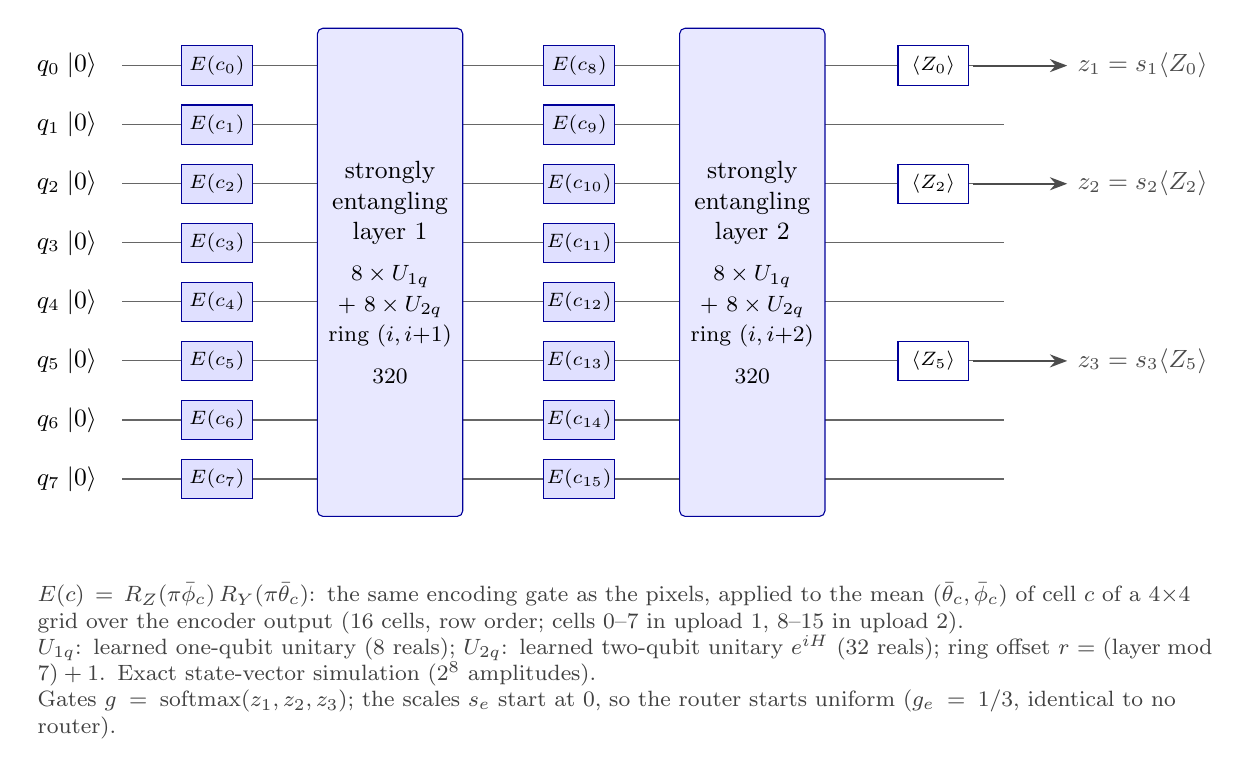
\begin{tikzpicture}[x=1cm, y=-0.75cm]
  \foreach \q in {0,...,7} {
    \node[anchor=east, font=\small] at (-0.2,\q) {$q_{\q}\;|0\rangle$};
    \draw[black!60] (0,\q) -- (11.2,\q);
  }
  % upload 1: cells 0-7
  \foreach \q in {0,...,7} { \node[gate] at (1.2,\q) {$E(c_{\q})$}; }
  \node[qbox, minimum width=18mm, minimum height=62mm] at (3.4,3.5) {strongly\\entangling\\layer 1\\[4pt]\footnotesize $8\times U_{1q}$\\ \footnotesize + $8\times U_{2q}$\\ \footnotesize ring $(i,i{+}1)$\\[4pt]\footnotesize 320};
  % upload 2: cells 8-15
  \foreach \q in {0,...,7} {
    \pgfmathtruncatemacro{\c}{\q+8}
    \node[gate] at (5.8,\q) {$E(c_{\c})$};
  }
  \node[qbox, minimum width=18mm, minimum height=62mm] at (8.0,3.5) {strongly\\entangling\\layer 2\\[4pt]\footnotesize $8\times U_{1q}$\\ \footnotesize + $8\times U_{2q}$\\ \footnotesize ring $(i,i{+}2)$\\[4pt]\footnotesize 320};
  % measurements
  \foreach \q/\e in {0/1, 2/2, 5/3} {
    \node[meas] at (10.3,\q) {$\langle Z_{\q}\rangle$};
    \draw[->, thick, black!70] (10.8,\q) -- (12.0,\q) node[right, font=\small] {$z_{\e} = s_{\e}\langle Z_{\q}\rangle$};
  }
  \node[note, anchor=north west, text width=150mm] at (-1.2,8.6) {%
    $E(c) = R_Z(\pi\bar\phi_c)\,R_Y(\pi\bar\theta_c)$: the same encoding gate as the pixels, applied to the mean $(\bar\theta_c,\bar\phi_c)$
    of cell $c$ of a $4{\times}4$ grid over the encoder output (16 cells, row order; cells $0$--$7$ in upload 1, $8$--$15$ in upload 2).\\
    $U_{1q}$: learned one-qubit unitary (8 reals); $U_{2q}$: learned two-qubit unitary $e^{iH}$ (32 reals); ring offset $r = (\text{layer} \bmod 7) + 1$.
    Exact state-vector simulation ($2^8$ amplitudes).\\
    Gates $g = \mathrm{softmax}(z_1,z_2,z_3)$; the scales $s_e$ start at 0, so the router starts uniform ($g_e = 1/3$, identical to no router).};
\end{tikzpicture}

\end{document}
